\section{Results}

\begin{figure}
  \begin{centering}
  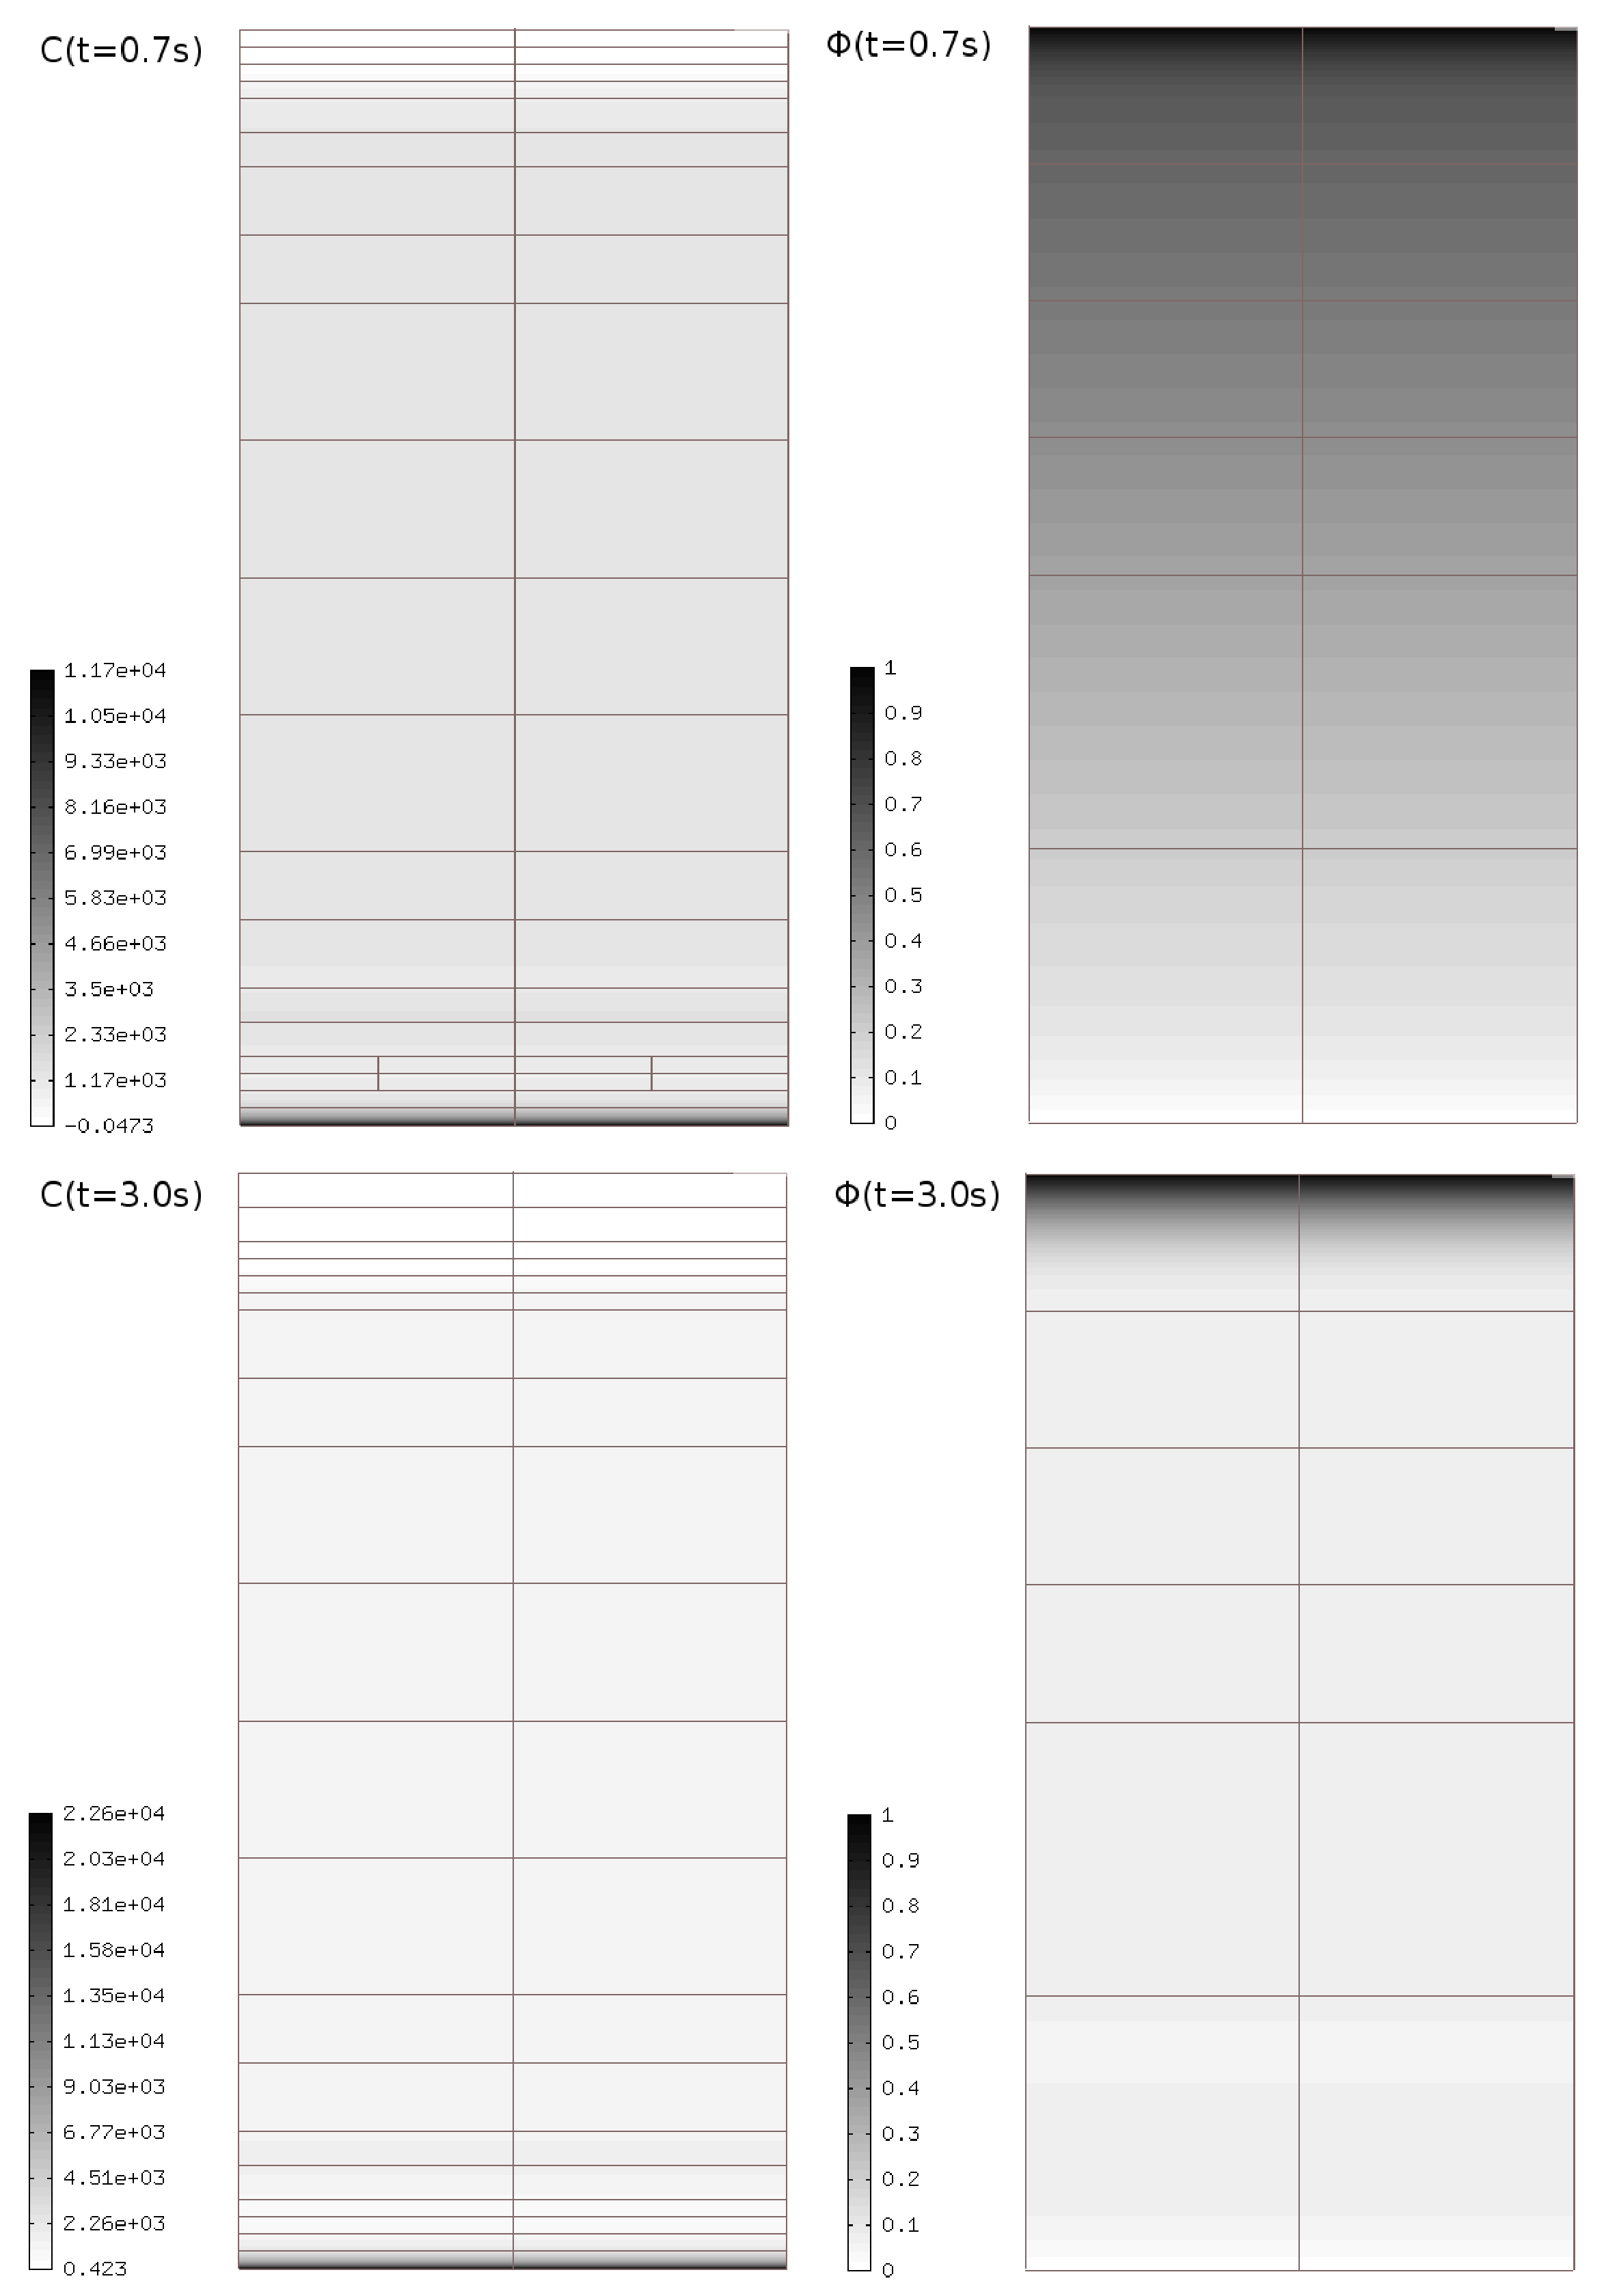
\includegraphics[width=.75\columnwidth]{cphi}
  \caption{\label{fig:cphi} Concentration $C$
  and voltage $\phi$ at two different time steps
  (HP\_ANISO adaptivity was used).}
  \end{centering}
\end{figure}

We ran the calculation for all the adaptivity types 
in both single-mesh and multi-mesh configurations. 
Example of the solution at $t=0.7\ s$ and $t=3.0\ s$ 
with adaptivity type HP\_ANISO is shown
in Fig.~\ref{fig:cphi}. The time $t=0.7\ s$ was chosen because
by that time, some ionic migration has already taken place, i.e.
concentration gradient near the $\partial\Omega_1$ and
$\partial\Omega_3$ has formed. The automatic mesh refinements
at different time steps are clearly visible --- especially
near the top boundary, where the concentration gradient is
moving in time (as seen in Fig.~\ref{fig:comsol-conc-volt}).

The following numeric results were recorded for each 
adaptivity type: converged error at each time step, cumulative CPU
time at each time step, and the problem size in terms of number
of degrees of freedoms (NDOFs) at each time step.  
Two types of initial meshes were used --- in case of only \emph{p}-adaptivity,
more refined mesh was used. When also the element size refinement
was enabled (all \emph{h} adaptivity types), very coarse initial mesh
was used. In any case, the initial mesh was loaded at each time step.


\begin{figure}
  \begin{centering}
  
\includegraphics[width=.8\columnwidth]{mesh}
  \caption{\label{fig:mesh} Initial coarse mesh (a),
  	half refined mesh (b) and refined mesh (c). The coarse mesh
	and refined mesh were used in the initial calcualtions, the latter one
	in case of \emph{p}-adaptivity (including HP\_ANISO\_P). The half-refined mesh was
	used later to optimize \emph{hp}-adaptive mode solutions.}
  \end{centering}
\end{figure}

Some initial observations
helped to select the graphs for this work --- it would have been unreasonable 
to present all recorded results for each adaptivity type.
First of all, the multi-mesh configuration resulted smaller problem size, faster
calculation, and better or similar error convergence than the single-mesh
configuration for all but HP\_ANISO\_H adaptivity type. In this case
the single-mesh configuration resulted slightly but not significantly
smaller problem size, therefore, single-mesh results of HP\_ANISO\_H
are considered in further comparisons. It must be also noted that in case of the isotropic
refinements, only P\_ISO adaptivity mode resulted in a reasonable problem size.
Secondly, H\_ISO did not converge very well in terms of the
calculation time and the problem size. The term ``reasonable problem size''
means that the number of degrees of freedom in time converges
to so that $N_{dof}<500$, and the term ``reasonable calculation time''
means that the calculation (step $\tau=0.01\ s$, physical
time $t_{end}=3.0\ s$) time $t$ on a givem system was $t<500\ s$.
Although these parameters are empirical, they serve as an upper limit, given
that the most adaptivity modes gave significantly smaller results,
e.g. $t<<500\ s$ and $N_{dof} << 500$.
Therefore, the multi-mesh calculation results H\_ISO, H\_ANSIO, P\_ANISO,
HP\_ANISO, HP\_ANISO\_P and the single-mesh calculation results of HP\_ANISO\_H
adaptivity mode will be compared. In all of the cases, the relative 
error at each time step remained below
the threshold which were set to $e_{th}=0.5\%$ between the coarse mesh
and fine mesh solutions.

\begin{figure}
  \begin{centering}
  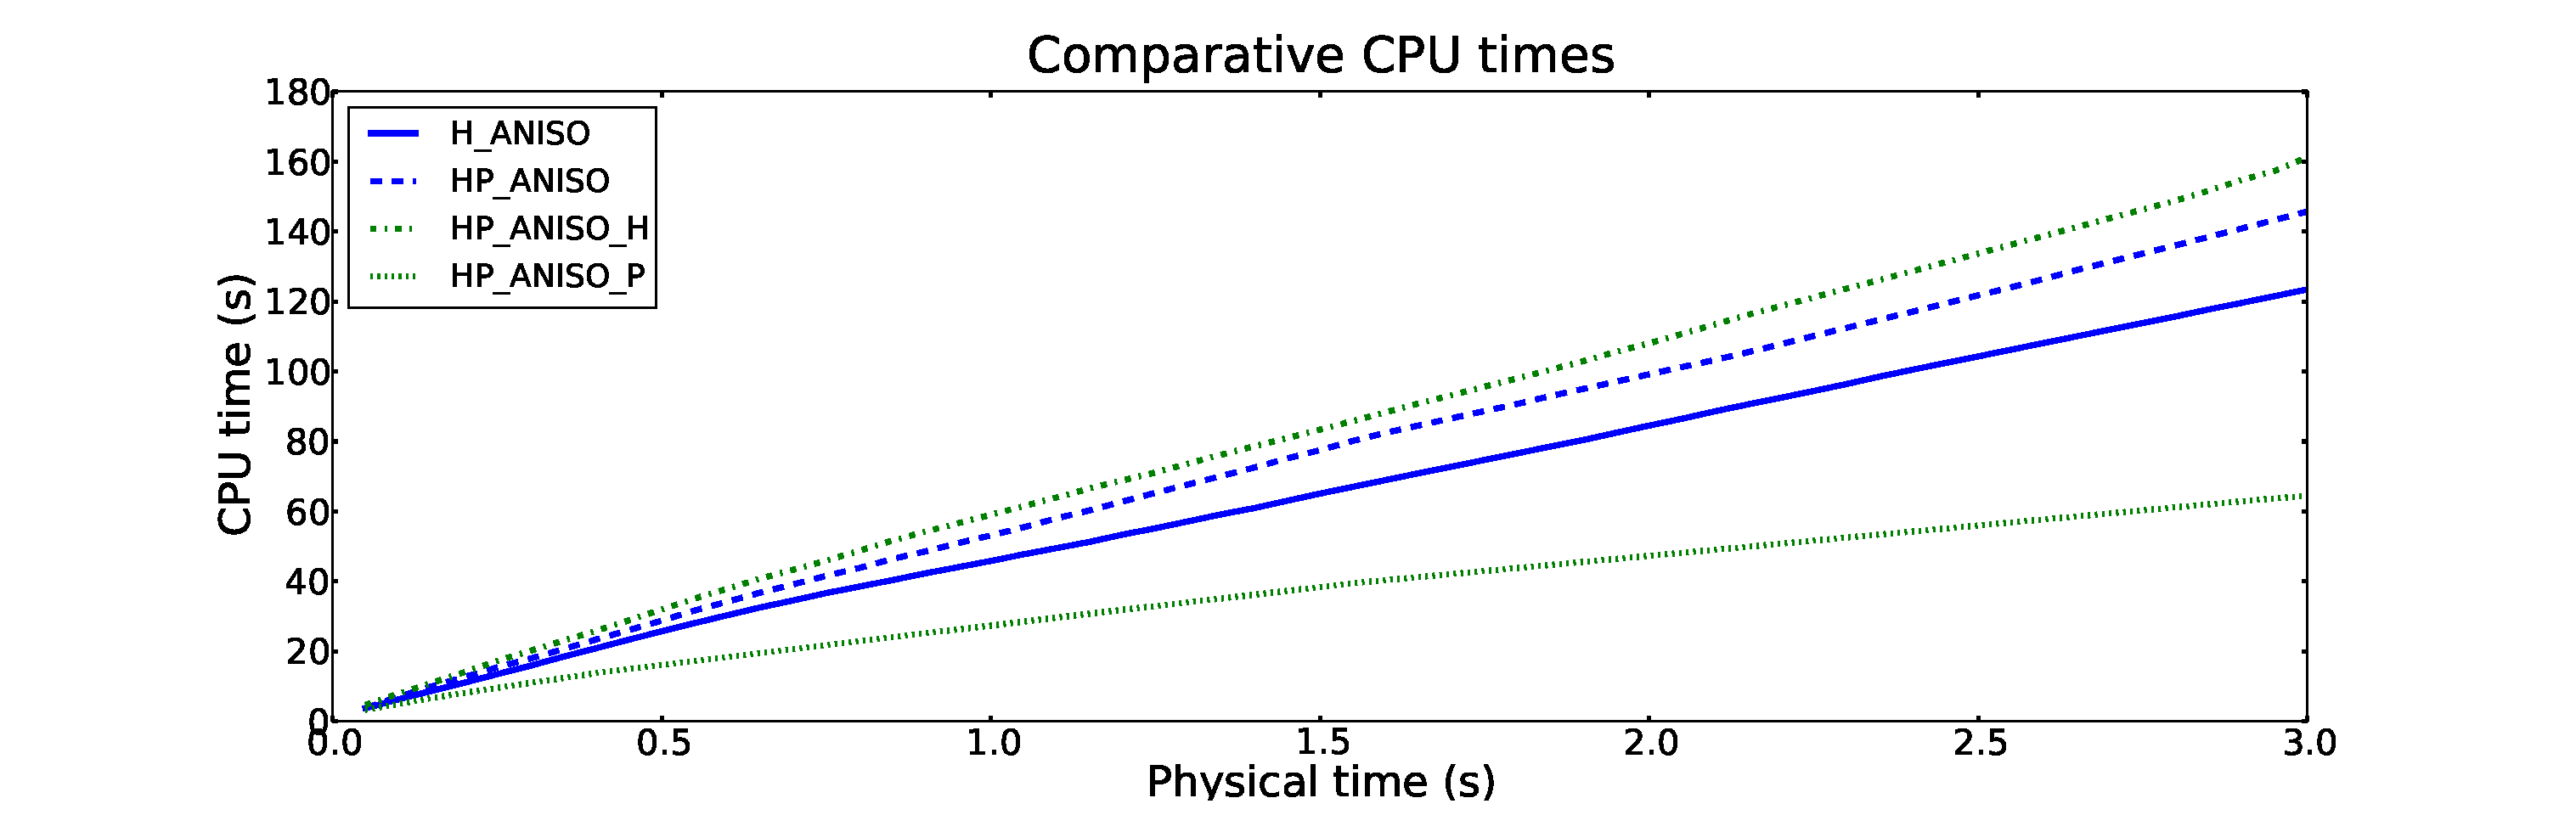
\includegraphics[width=\columnwidth]{cpu}
  \caption{\label{fig:cpu} Cumulative CPU time for different adaptivity modes.}
  \end{centering}
\end{figure}

\begin{figure}
  \begin{centering}
  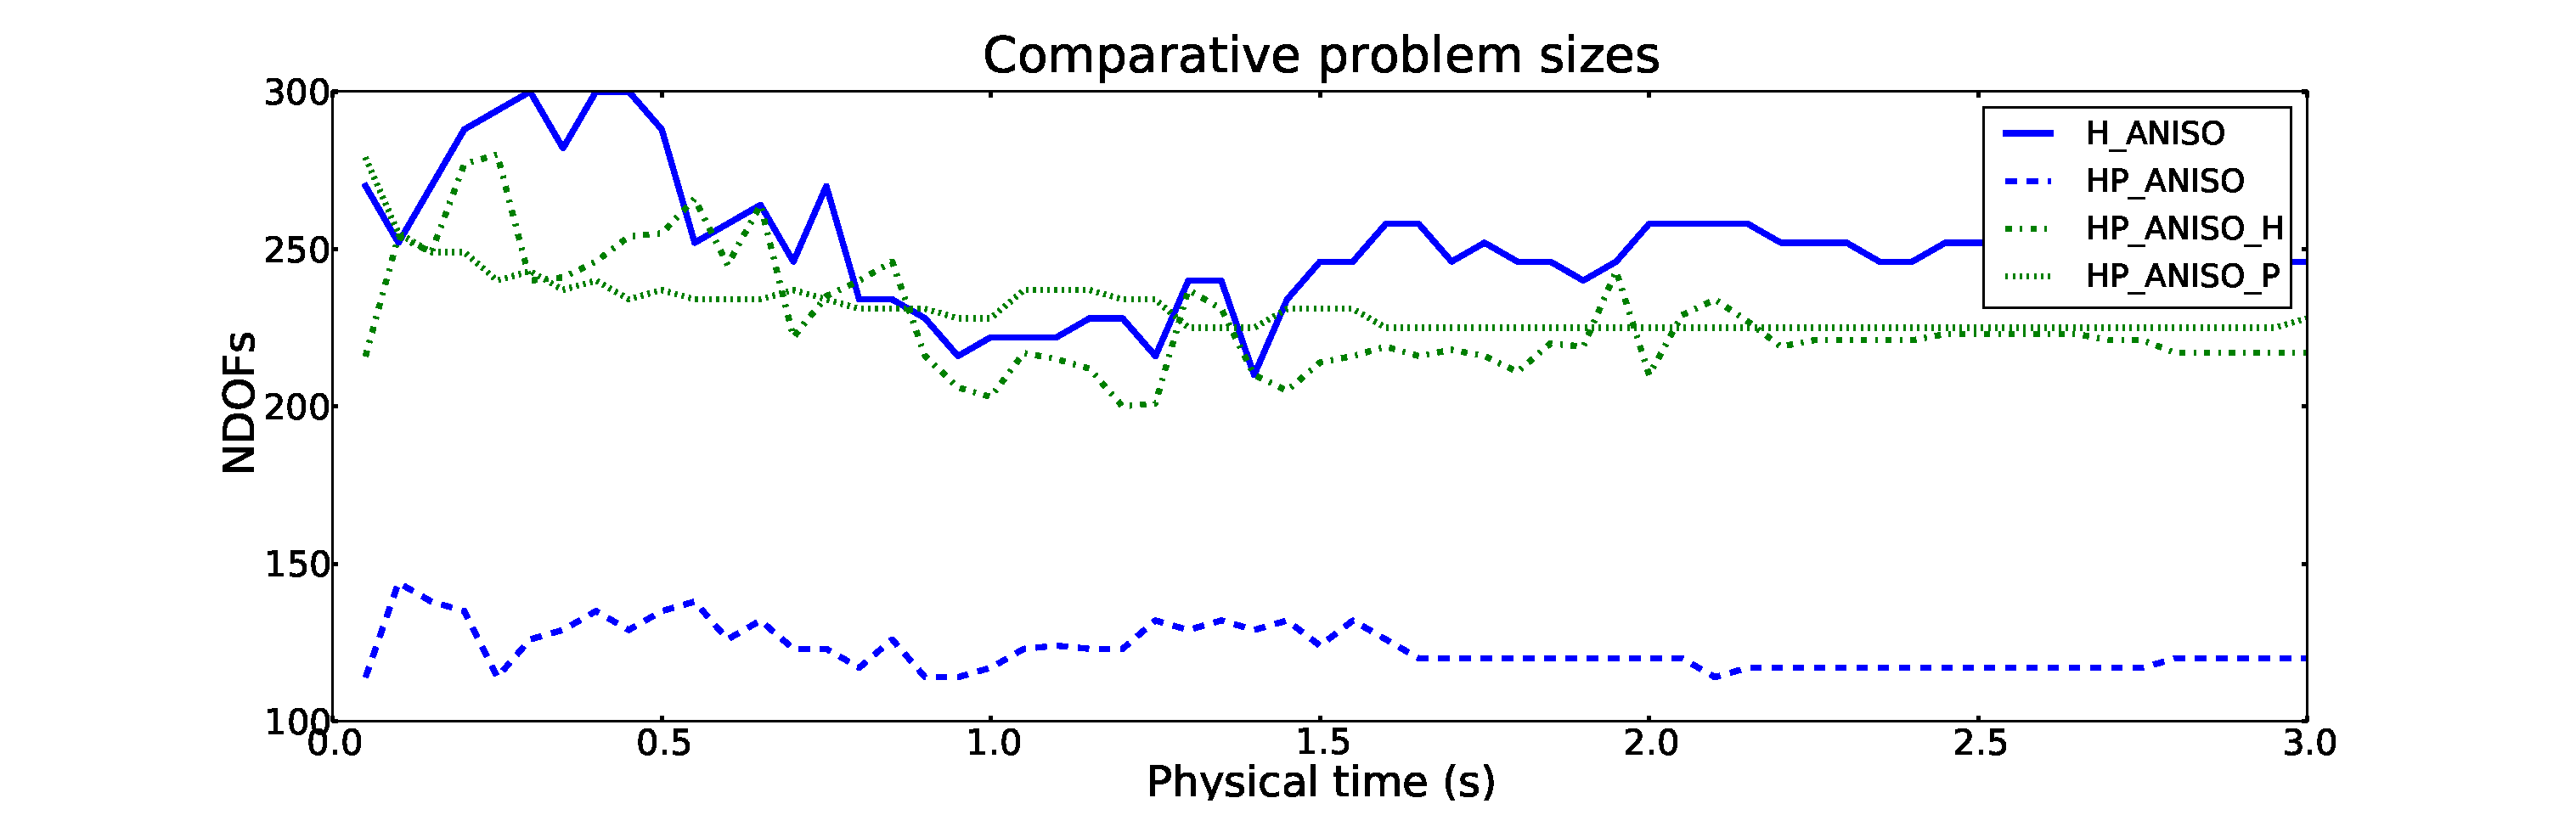
\includegraphics[width=\columnwidth]{dof}
  \caption{\label{fig:dof} NDOFs at each time step for different adaptivity modes.}
  \end{centering}
\end{figure}

Fig.~\ref{fig:cpu} shows the cumulative CPU time for different adaptivity
modes at each time step. All the calculations were done on the same computer.
Here we see that HP\_ANISO requires the most
resources which can be understood from the fact that this adaptivity mode has the largest number of 
candidates (see XXX) from which the refinement methode is chosen.
At the same time, HP\_ANISO\_H is the fastest.
Fig.~\ref{fig:dof} shows the NDOFs at each time step for different adaptivity modes.
There we see that the HP\_ANISO results in the smallest problem size --- $N_{dof} \approx 125$. 
All the other adaptivity modes result in  the problem size approximately ($N_{dof} \approx 300$), 
however, \emph{p}-adaptivity modes P\_ISO and P\_ANISO start off with relatively large $N_{dof}$.
We can see from the graphs and also from the Fig.~\ref{fig:mesh} that
\emph{p}-adaptivity is used for the most part of the problem. The initially high
$N_{dof}$ for \emph{p}-adaptive modes indicate that only first time steps benefit
greatly from the \emph{h}-adaptivity. P\_ISO, HP\_ANISO\_H
and HP\_ANISO\_P are the fastest in terms of CPU time, however, we have to consider
that P\_ISO  and HP\_ANISO\_P start off from more refined mesh.

\begin{figure}
  \begin{centering}
  \includegraphics[width=\columnwidth]{refined_cpu}
  \caption{\label{fig:refined-cpu} Cumulative CPU time for HP\_ANISO and HP\_ANISO\_P
  with different initial meshes.}
  \end{centering}
\end{figure}

\begin{figure}
  \begin{centering}
  \includegraphics[width=\columnwidth]{refined_dof}
  \caption{\label{fig:refined-dof} NDOFs at each time step for
  HP\_ANISO and HP\_ANISO\_P with different meshes.}
  \end{centering}
\end{figure}

So far we have seen that HP\_ANISO results in the smallest problem size, but takes
most CPU time. When it comes to a large domain or 3D modeling the problem
size becomes the most important factor. Therefore, we consider HP\_ANISO the most
suitable adaptivity type to the given problem. Thus some ways to optimize the time
factor was considered. We neglected HP\_ANISO\_H as this uses single mesh only
and for large 3D domains, we believe the multi-mesh approach would be
more reasonable. The performance of HP\_ANISO\_P with refined mesh and half-refined
mesh, and performance of HP\_ANISO with unrefined, half-refined, and refined
meshes was calculated (see Fig.~\ref{fig:mesh}).
The results are shown in Fig.~\ref{fig:refined-cpu} and Fig.~\ref{fig:refined-dof}.

TODO(more explanation) It can be seen that some initial refinemts help to reduce the CPU time,
however, it increases the problem size.
